\section{双曲函数、反双曲函数}
\begin{definition}[双曲函数]
\begin{gather}
	\sinh x \defeq \frac{e^x - e^{-x}}2. \\
	\cosh x \defeq \frac{e^x + e^{-x}}2. \\
	\tanh x \defeq \frac{\sinh x}{\cosh x}. \\
	\coth x \defeq \frac{\cosh x}{\sinh x}. \\
	\sech x \defeq \frac1{\cosh x}. \\
	\csch x \defeq \frac1{\sinh x}.
\end{gather}
这里,
\(\sinh x\)被称为\DefineConcept{双曲正弦},
\(\cosh x\)被称为\DefineConcept{双曲余弦},
\(\tanh x\)被称为\DefineConcept{双曲正切},
\(\coth x\)被称为\DefineConcept{双曲余切}.
\end{definition}

可以看出\begin{gather*}
	\tanh x = \frac{e^x - e^{-x}}{e^x + e^{-x}}. \\
	\coth x = \frac{e^x + e^{-x}}{e^x - e^{-x}}.
\end{gather*}

\begin{figure}[htb]
	\centering
	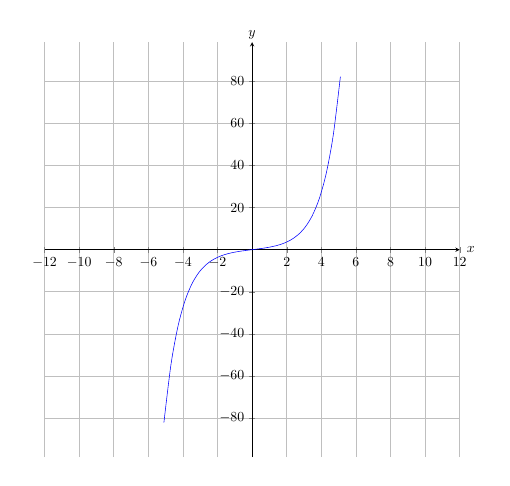
\begin{tikzpicture}[scale=.5]
		\begin{axis}[
			xmin=-10,xmax=10,
			restrict y to domain=-100:100,
			grid=both,width=\textwidth,height=\textwidth,
			axis lines=middle,
			xlabel=$x$,
			ylabel=$y$,
			enlarge x limits=0.1,
			enlarge y limits=0.1,
			x label style={at={(ticklabel* cs:1.00)}, inner sep=5pt, anchor=west},
			y label style={at={(ticklabel* cs:1.00)}, inner sep=2pt, anchor=south},
		]
			\addplot[color=blue,samples=50,smooth,domain=-10:10]{.5*(exp(x)-exp(-x))};
		\end{axis}
	\end{tikzpicture}
	\caption{双曲正弦函数\(\sinh\)的图形}
	\label{figure:函数.双曲正弦函数的图形}
\end{figure}
%@Mathematica: Plot[Sinh[x], {x, -10, 10}]

\begin{figure}[htb]
	\centering
	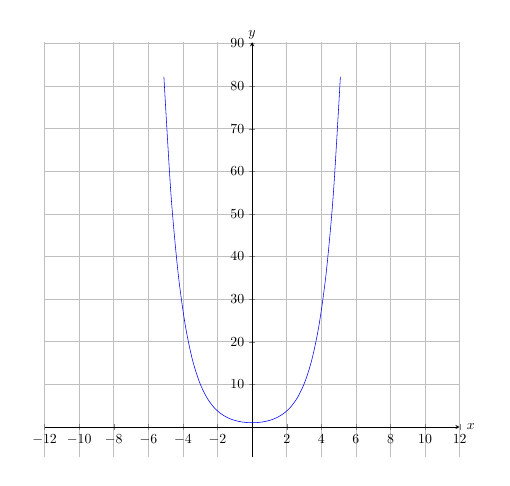
\begin{tikzpicture}[scale=.5]
		\begin{axis}[
			xmin=-10,xmax=10,
			restrict y to domain=-100:100,
			grid=both,width=\textwidth,height=\textwidth,
			axis lines=middle,
			xlabel=$x$,
			ylabel=$y$,
			enlarge x limits=0.1,
			enlarge y limits=0.1,
			x label style={at={(ticklabel* cs:1.00)}, inner sep=5pt, anchor=west},
			y label style={at={(ticklabel* cs:1.00)}, inner sep=2pt, anchor=south},
		]
			\addplot[color=blue,samples=50,smooth,domain=-10:10]{.5*(exp(x)+exp(-x))};
		\end{axis}
	\end{tikzpicture}
	\caption{双曲余弦函数\(\cosh\)的图形}
	\label{figure:函数.双曲余弦函数的图形}
\end{figure}
%@Mathematica: Plot[Cosh[x], {x, -10, 10}]

\begin{figure}[htb]
	\centering
	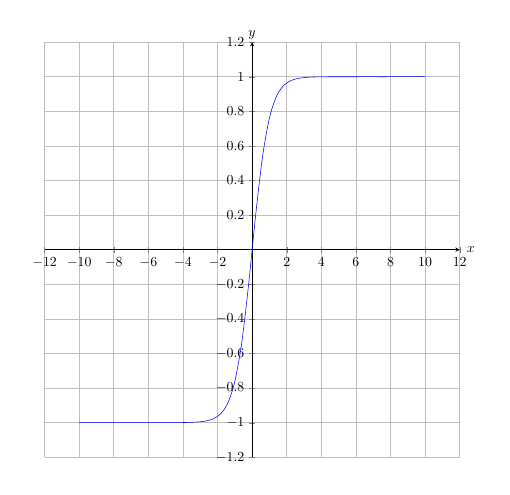
\begin{tikzpicture}[scale=.5]
		\begin{axis}[
			xmin=-10,xmax=10,
			restrict y to domain=-100:100,
			grid=both,width=\textwidth,height=\textwidth,
			axis lines=middle,
			xlabel=$x$,
			ylabel=$y$,
			enlarge x limits=0.1,
			enlarge y limits=0.1,
			x label style={at={(ticklabel* cs:1.00)}, inner sep=5pt, anchor=west},
			y label style={at={(ticklabel* cs:1.00)}, inner sep=2pt, anchor=south},
		]
			\addplot[color=blue,samples=50,smooth,domain=-10:10]{(exp(x)-exp(-x))/(exp(x)+exp(-x))};
		\end{axis}
	\end{tikzpicture}
	\caption{双曲正切函数\(\tanh\)的图形}
	\label{figure:函数.双曲正切函数的图形}
\end{figure}
%@Mathematica: Plot[Tanh[x], {x, -10, 10}]

\begin{figure}[htb]
	\centering
	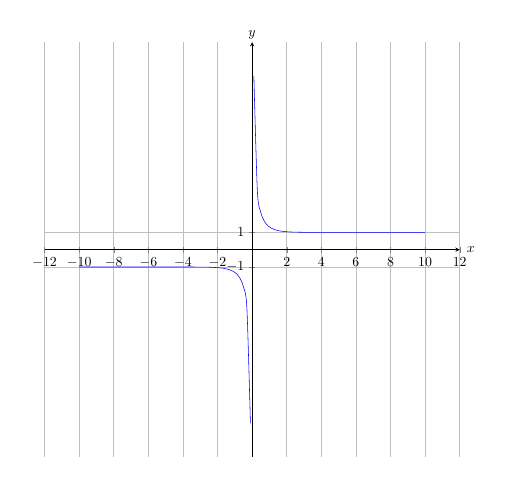
\begin{tikzpicture}[scale=.5]
		\begin{axis}[
			xmin=-10,xmax=10,
			ymin=-10,ymax=10,
			grid=both,width=\textwidth,height=\textwidth,
			axis lines=middle,
			xlabel=$x$,
			ylabel=$y$,
			enlarge x limits=0.1,
			enlarge y limits=0.1,
			x label style={at={(ticklabel* cs:1.00)}, inner sep=5pt, anchor=west},
			y label style={at={(ticklabel* cs:1.00)}, inner sep=2pt, anchor=south},
			ytick={-1,1},
		]
			\addplot[color=blue,samples=50,smooth,domain=-10:-.1]
				{(exp(x)+exp(-x))/(exp(x)-exp(-x))};
			\addplot[color=blue,samples=50,smooth,domain=.1:10]
				{(exp(x)+exp(-x))/(exp(x)-exp(-x))};
		\end{axis}
	\end{tikzpicture}
	\caption{双曲余切函数\(\coth\)的图形}
	\label{figure:函数.双曲余切函数的图形}
\end{figure}
%@Mathematica: Plot[Coth[x], {x, -10, 10}]

\begin{figure}[htb]
	\centering
	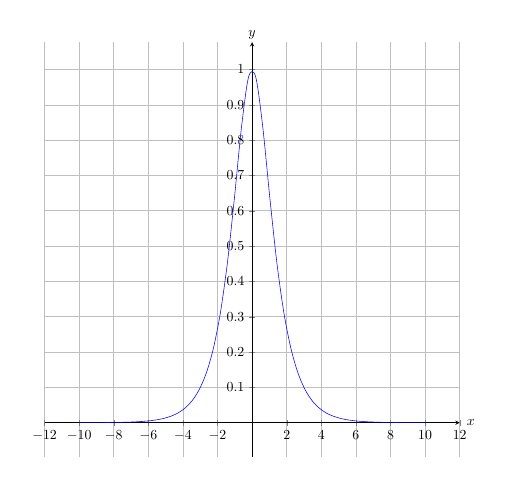
\begin{tikzpicture}[scale=.5]
		\begin{axis}[
			xmin=-10,xmax=10,
			restrict y to domain=-100:100,
			grid=both,width=\textwidth,height=\textwidth,
			axis lines=middle,
			xlabel=$x$,
			ylabel=$y$,
			enlarge x limits=0.1,
			enlarge y limits=0.1,
			x label style={at={(ticklabel* cs:1.00)}, inner sep=5pt, anchor=west},
			y label style={at={(ticklabel* cs:1.00)}, inner sep=2pt, anchor=south},
		]
			\addplot[color=blue,samples=50,smooth,domain=-10:10]{2/(exp(x)+exp(-x))};
		\end{axis}
	\end{tikzpicture}
	\caption{双曲正割函数\(\sech\)的图形}
\end{figure}
%@Mathematica: Plot[Sech[x], {x, -10, 10}]

\begin{figure}[htb]
	\centering
	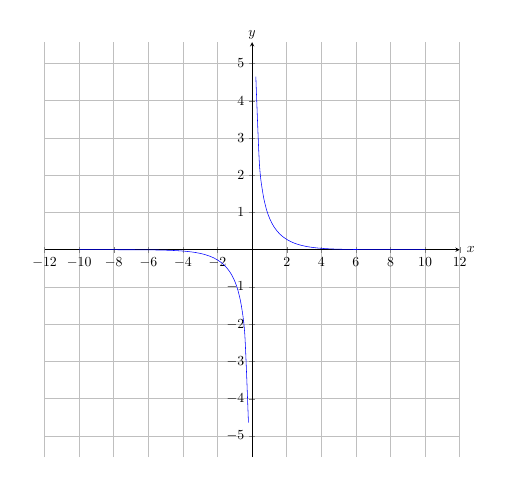
\begin{tikzpicture}[scale=.5]
		\begin{axis}[
			xmin=-10,xmax=10,
			restrict y to domain=-100:100,
			grid=both,width=\textwidth,height=\textwidth,
			axis lines=middle,
			xlabel=$x$,
			ylabel=$y$,
			enlarge x limits=0.1,
			enlarge y limits=0.1,
			x label style={at={(ticklabel* cs:1.00)}, inner sep=5pt, anchor=west},
			y label style={at={(ticklabel* cs:1.00)}, inner sep=2pt, anchor=south},
		]
			\addplot[color=blue,samples=50,smooth,domain=-10:-.01]{2/(exp(x)-exp(-x))};
			\addplot[color=blue,samples=50,smooth,domain=.01:10]{2/(exp(x)-exp(-x))};
		\end{axis}
	\end{tikzpicture}
	\caption{双曲余割函数\(\csch\)的图形}
\end{figure}
%@Mathematica: Plot[Csch[x], {x, -10, 10}]

下面我们研究双曲函数的反函数.

首先讨论双曲正弦\(y=\sinh x\)的反函数.
由\(x=\sinh y\),有\begin{equation*}
	x=\frac{e^y-e^{-y}}{2}.
\end{equation*}
令\(u=e^y\),则有\begin{equation*}
	u^2-2xu-1=0.
\end{equation*}
这是一个关于\(u\)的一元二次方程,解得\begin{equation*}
	u=x\pm\sqrt{x^2+1}.
\end{equation*}
因为\(u=e^y>0\),故上式根号前应取正号,即\begin{equation*}
	u=x+\sqrt{x^2+1}.
\end{equation*}
又由\(y=\ln u\),故得反双曲正弦\begin{equation*}
	\arsinh x
	\defeq
	\ln(x+\sqrt{x^2+1}),
	\quad -\infty<x<+\infty.
\end{equation*}

\begin{figure}[htb]
	\centering
	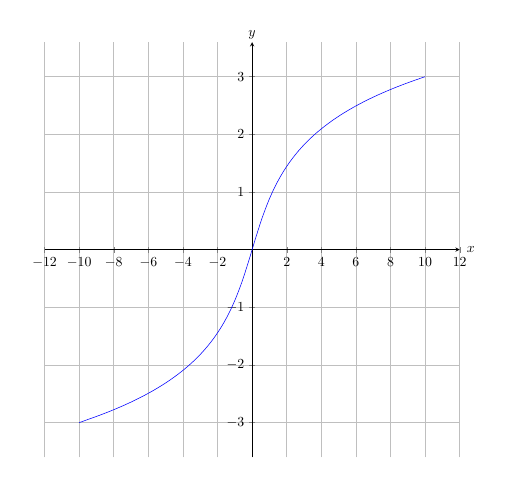
\begin{tikzpicture}[scale=.5]
		\begin{axis}[
			xmin=-10,xmax=10,
			restrict y to domain=-100:100,
			grid=both,width=\textwidth,height=\textwidth,
			axis lines=middle,
			xlabel=$x$,
			ylabel=$y$,
			enlarge x limits=0.1,
			enlarge y limits=0.1,
			x label style={at={(ticklabel* cs:1.00)}, inner sep=5pt, anchor=west},
			y label style={at={(ticklabel* cs:1.00)}, inner sep=2pt, anchor=south},
		]
			\addplot[color=blue,samples=50,smooth,domain=-10:10]{ln(x+sqrt(1+x^2))};
		\end{axis}
	\end{tikzpicture}
	\caption{反双曲正弦函数\(\arsinh\)的图形}
\end{figure}
%@Mathematica: Plot[ArcSinh[x], {x, -10, 10}]

接下来讨论双曲余弦函数\(y=\cosh x\)的反函数.
由\(x=\cosh y\),有\begin{equation*}
	x=\frac{e^y+e^{-y}}{2},
\end{equation*}
显然恒有\(x>0\).
由此得\(e^y=x\pm\sqrt{x^2-1}\ (x\geq1)\),
故\begin{equation*}
	y=\ln(x\pm\sqrt{x^2-1})
	\quad(x\geq1).
\end{equation*}
可见,函数\begin{equation*}
	y=\ln(x+\sqrt{x^2-1})
	\quad(x\geq1)
\end{equation*}是双曲余弦函数右支\(y=\cosh x\ (x\geq0)\)的反函数,
我们把它记作\(\arcosh x\),
即\begin{equation*}
	\arcosh x
	\defeq
	\ln(x + \sqrt{x^2 - 1}),
	\quad 1\leq x<+\infty.
\end{equation*}
而函数\begin{equation*}
	y=\ln(x-\sqrt{x^2-1})
	\quad(x\geq1)
\end{equation*}是双曲余弦函数左支\(y=\cosh x\ (x\leq0)\)的反函数.

\begin{figure}[htb]
	\centering
	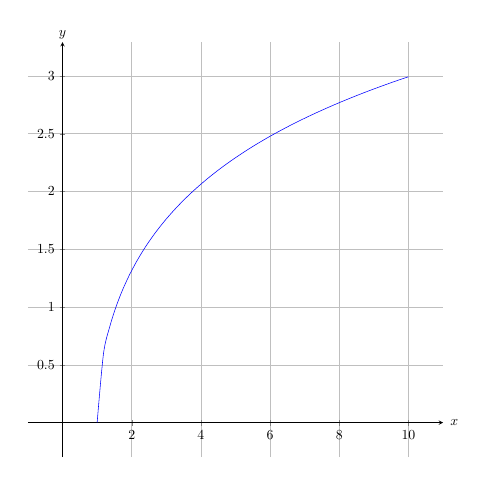
\begin{tikzpicture}[scale=.5]
		\begin{axis}[
			xmin=0,xmax=10,
			restrict y to domain=-100:100,
			grid=both,width=\textwidth,height=\textwidth,
			axis lines=middle,
			xlabel=$x$,
			ylabel=$y$,
			enlarge x limits=0.1,
			enlarge y limits=0.1,
			x label style={at={(ticklabel* cs:1.00)}, inner sep=5pt, anchor=west},
			y label style={at={(ticklabel* cs:1.00)}, inner sep=2pt, anchor=south},
		]
			\addplot[color=blue,samples=50,smooth,domain=1:10]{ln(x+sqrt(x^2-1))};
		\end{axis}
	\end{tikzpicture}
	\caption{反双曲余弦函数\(\arcosh\)的图形}
\end{figure}
%@Mathematica: Plot[ArcCosh[x], {x, 0, 10}]

易见\begin{equation*}
	\ln(x+\sqrt{x^2-1}) + \ln(x-\sqrt{x^2-1}) = 0
	\quad(x\geq1).
\end{equation*}
%@Mathematica: FullSimplify[Log[x + Sqrt[x^2 - 1]] + Log[x - Sqrt[x^2 - 1]], Assumptions -> {x >= 1}]
%@credit: {cee35532-e299-4587-89a0-7b84e7454774}

然后讨论双曲正切函数\(\tanh\)的反函数.
由\begin{equation*}
	x = \tanh y
	= \frac{e^y-e^{-y}}{e^y+e^{-y}}
	= \frac{e^{2y}-1}{e^{2y}+1},
\end{equation*}得\begin{equation*}
	(1-x) e^{2y} = 1+x,
\end{equation*}
解得\(y = \frac12 \ln\frac{1+x}{1-x}\).
要使对数\(\ln\frac{1+x}{1-x}\)有意义,必有\((1+x)(1-x)>0\),
即\(x\in(-1,1)\).
于是反双曲正切函数可以定义为\begin{equation*}
	\artanh x
	\defeq
	\frac12 \ln\frac{1 + x}{1 - x},
	\quad -1<x<1.
\end{equation*}

\begin{figure}[htb]
	\centering
	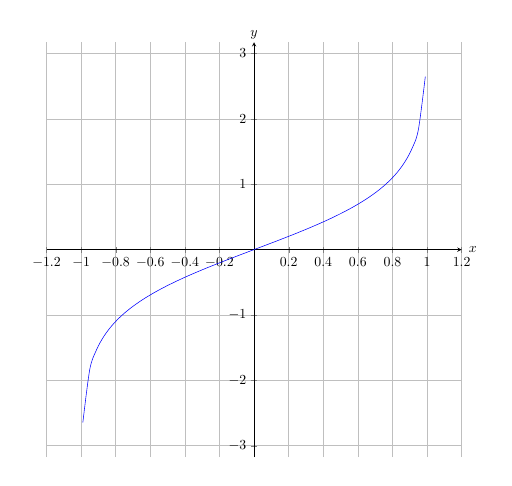
\begin{tikzpicture}[scale=.5]
		\begin{axis}[
			xmin=-1,xmax=1,
			restrict y to domain=-100:100,
			grid=both,width=\textwidth,height=\textwidth,
			axis lines=middle,
			xlabel=$x$,
			ylabel=$y$,
			enlarge x limits=0.1,
			enlarge y limits=0.1,
			x label style={at={(ticklabel* cs:1.00)}, inner sep=5pt, anchor=west},
			y label style={at={(ticklabel* cs:1.00)}, inner sep=2pt, anchor=south},
		]
			\addplot[color=blue,samples=50,smooth,domain=-.99:.99]{.5*ln((1+x)/(1-x))};
		\end{axis}
	\end{tikzpicture}
	\caption{反双曲正切函数\(\artanh\)的图形}
\end{figure}
%@Mathematica: Plot[ArcTanh[x], {x, -1, 1}]

最后讨论双曲余切函数\(\coth\)的反函数.
由\begin{equation*}
	x = \coth y
	= \frac{e^y+e^{-y}}{e^y-e^{-y}}
	= \frac{e^{2y}+1}{e^{2y}-1},
\end{equation*}得\begin{equation*}
	(x-1) e^{2y} = 1+x,
\end{equation*}
解得\(y = \frac12 \ln\frac{x+1}{x-1}\).
要使对数\(\ln\frac{x+1}{x-1}\)有意义,必有\((x+1)(x-1)>0\),
即\(x\in(-\infty,-1)\cup(1,+\infty)\).
于是反双曲余切函数可以定义为\begin{equation*}
	\arcoth x
	\defeq
	\frac12 \ln\frac{x + 1}{x - 1},
	\quad -\infty<x<-1\lor1<x<+\infty.
\end{equation*}

\begin{figure}[htb]
	\centering
	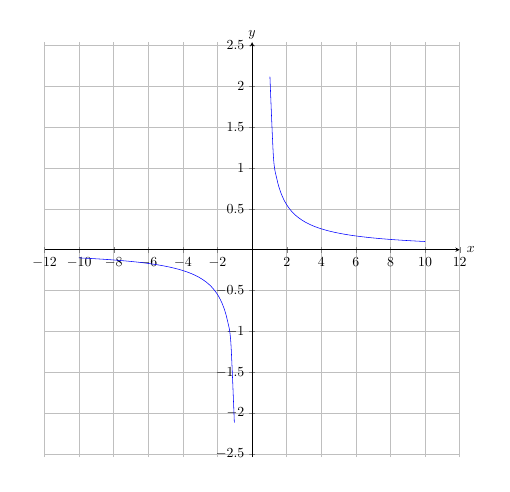
\begin{tikzpicture}[scale=.5]
		\begin{axis}[
			xmin=-10,xmax=10,
			restrict y to domain=-100:100,
			grid=both,width=\textwidth,height=\textwidth,
			axis lines=middle,
			xlabel=$x$,
			ylabel=$y$,
			enlarge x limits=0.1,
			enlarge y limits=0.1,
			x label style={at={(ticklabel* cs:1.00)}, inner sep=5pt, anchor=west},
			y label style={at={(ticklabel* cs:1.00)}, inner sep=2pt, anchor=south},
		]
			\addplot[color=blue,samples=50,smooth,domain=-10:-.01]{.5*ln((x+1)/(x-1))};
			\addplot[color=blue,samples=50,smooth,domain=.01:10]{.5*ln((x+1)/(x-1))};
		\end{axis}
	\end{tikzpicture}
	\caption{反双曲余切函数\(\arcoth\)的图形}
\end{figure}
%@Mathematica: Plot[ArcCoth[x], {x, -10, 10}]

\begin{property}
双曲正弦\(\sinh\)是奇函数.
\end{property}

\begin{property}
双曲余弦\(\cosh\)是偶函数.
\end{property}

\begin{property}
\(\cosh x\)有下界:\begin{equation*}
	\cosh x \geq 1
\end{equation*}
当且仅当\(x=0\)时,上式取等号.
\end{property}

\begin{theorem}
\begin{gather}
	\sinh(x \pm y) = \sinh x\cosh y \pm \cosh x\sinh y, \\
	\cosh(x \pm y) = \cosh x\cosh y \pm \sinh x\sinh y, \\
	\tanh(x + y) = \frac{\tanh x + \tanh y}{1 + \tanh x\tanh y}.
\end{gather}
\begin{proof}
根据双曲函数的定义有
\begin{align*}
	\sinh x\cosh y+\cosh x\sinh y
	&= \frac{e^x - e^{-x}}{2} \frac{e^y + e^{-y}}{2}
		+ \frac{e^x + e^{-x}}{2} \frac{e^y - e^{-y}}{2} \\
	&= \frac{1}{4} (e^x e^y + e^x e^{-y} - e^{-x} e^y - e^{-x} e^{-y} \\
	&\qquad+ e^x e^y - e^x e^{-y} + e^{-x} e^y - e^{-x} e^{-y}) \\
	&= \frac{1}{4} (2 e^x e^y - 2 e^{-x} e^{-y}) \\
	&= \frac12 (e^{x+y} - e^{-x-y}) = \sinh(x+y).
\end{align*}
\begin{align*}
	\cosh x\cosh y+\sinh x\sinh y
	&= \frac{e^x + e^{-1}}{2} \frac{e^y + e^{-y}}{2}
		+ \frac{e^x - e^{-x}}{2} \frac{e^y - e^{-y}}{2} \\
	&= \frac{1}{4} (e^x e^y + e^x e^{-y} + e^{-x} e^y + e^{-x} e^{-y} \\
	&\qquad+ e^x e^y - e^x e^{-y} - e^{-x} e^y + e^{-x} e^{-y}) \\
	&= \frac{1}{4} (2 e^x e^y + 2 e^{-x} e^{-y}) \\
	&= \frac12 (e^{x+y} + e^{-x-y}) = \cosh(x+y).
	\qedhere
\end{align*}
\end{proof}
\end{theorem}

\begin{theorem}
\begin{gather}
	\cosh^2x - \sinh^2x = 1, \\
	\sinh x + \cosh x = e^x, \\
	\cosh x - \sinh x = e^{-x}, \\
	1 - \tanh^2 x = \sech^2 x, \\
	\coth^2 x - 1 = \csch^2 x.
\end{gather}
\begin{proof}
根据双曲函数的定义有
\begin{align*}
	\cosh^2x-\sinh^2x
	&=\left(\frac{e^x + e^{-x}}{2}\right)^2-\left(\frac{e^x - e^{-x}}{2}\right)^2 \\
	&=\frac{e^{2x}+2+e^{-2x}}{4}-\frac{e^{2x}-2+e^{-2x}}{4}
	=1.
	\qedhere
\end{align*}
\end{proof}
\end{theorem}

\begin{theorem}
\begin{gather}
	\sinh2x = 2 \sinh x\cosh x, \\
	\cosh2x = \cosh^2x + \sinh^2x.
\end{gather}
\end{theorem}
